	\documentclass[10pt,oneside]{CBFT_book}
	% Algunos paquetes
	\usepackage{amssymb}
	\usepackage{amsmath}
	\usepackage{graphicx}
% 	\usepackage{libertine}
% 	\usepackage[bold-style=TeX]{unicode-math}
	\usepackage{lipsum}

	\usepackage{natbib}
	\setcitestyle{square}

	\usepackage{polyglossia}
	\setdefaultlanguage{spanish}
	



	\usepackage{CBFT.estilo} % Cargo la hoja de estilo

	% Tipografías
	% \setromanfont[Mapping=tex-text]{Linux Libertine O}
	% \setsansfont[Mapping=tex-text]{DejaVu Sans}
	% \setmonofont[Mapping=tex-text]{DejaVu Sans Mono}

	%===================================================================
	%	DOCUMENTO PROPIAMENTE DICHO
	%===================================================================

\begin{document}

% =================================================================================================
\chapter{Introducción}
% =================================================================================================

Este capítulo es una introducción al formalismo.
Recordemos que el curso se basó fuertemente en el libro de Jon Jun Sakurai [bien escrito?].
La mecánica cuántica relativista desemboca en la teoría de campos.
Decir quizás que hay que, de alguna manera, olvidar todo lo anterior de la física clásica (hasta
nuevo aviso) porque esto conviene pensarlo de otra manera, será más abstracto.
Los sistemas, que serán muy sencillos, tendrán propiedades muy particulares, que luego se
conectarán con la física clásica en el límite apropiado.
La mecánica cuántica relativista añade más información además de corregir la clásica.

% =================================================================================================
\section{El experimento de Stern-Gerlach}
% =================================================================================================

Un horno emite átomos de plata (Ag) neutros con un electrón $e$ en la última órbita que le da el spín
al átomo como un todo. Al salir del horno los átomos tienen su spín orientado en cualquier dirección.
Ver figura.
El momento magnético del átomo que sale del horno es 
\[
	\vb{\mu} = \frac{e}{m_e c} \vb{S}
\]
donde acá está metido el magnetón de Bohr 
\[
	\mu_B = -\frac{ e \hbar }{2 m_e c}.
\]

\begin{figure}[htb]
	\begin{center}
	\includegraphics[width=0.9\textwidth]{images/teo2_1.pdf}	 
	\end{center}
	\caption{}
\end{figure} 

La fuerza $f_z$ que le ejerce el campo \vb{B} a estos átomos es 
\[
	f_z \propto - \mu_z
\]
de modo que el dispositivo SG mide y filtra por $S_z(\mu_z)$. Si el spín es un ente clásico
es de esperar un patrón como el sombreado en azul, pero se obtienen dos manchas; 
\notamargen{Uso átomos de plata que son neutros eléctricamente así no tengo efecto Hall.}
con la correspondencia mostrada bajo estas líneas
\begin{figure}[htb]
	\begin{center}
	\includegraphics[width=0.4\textwidth]{images/teo2_2.pdf}	 
	\end{center}
	\caption{}
\end{figure} 

Entonces el spín no es un ente {\it continuo}: está cuantizado y sólo puede tomar dos valores.
Llamamos a estos estados
\[
	(S_z,+) \qquad \qquad (S_z,-)
\]
Luego, un aparato de SG filtra o selecciona ciertos átomos. Podemos combinarlos.

\begin{figure}[htb]
	\begin{center}
	\includegraphics[width=0.6\textwidth]{images/teo2_3.pdf}	 
	\end{center}
	\caption{}
\end{figure} 

Con el dispositivo segundo orientado en $\hat{x}$ obtenemos mitad de átomos en
$(S_z,+)$ y mitad en $(S_z,-)$. La única es que en realidad lo que sucede es que 
$(S_z,+)$ se compone de $(S_x,+)$ y $(S_x,-)$.

Acá abajo sale $(S_z,-)$ pero para que ello sea posible 
$(S_x,+)$ se debe componer de $(S_z,+)$ y $(S_z,-)$. Pero esto no es posible
porque al segundo aparato no entró jamás $(S_z,-)$. Se filtró antes.

Los spines en $S_x, S_z$ son incompatibles entre sí. Al seleccionar $(S_z,+)$ en el segundo
SG se destruye la información previa sobre $S_z$. No podemos ya garantizar que $S_z$
sea nula.
\notamargen{Al medir uno la información cuántica del otro se pierde.}
El tercer experimento da al traste con la idea de que podamos pensar en spín como un
ente vectorial en 3D. Mediante una analogía con polarización de luz vemos que es necesario
meter al spín es un espacio vectorial de dimensión 2 pero con coeficientes complejos.

\begin{figure}[htb]
	\begin{center}
	\includegraphics[width=0.6\textwidth]{images/teo2_4.pdf}	 
	\end{center}
	\caption{}
\end{figure} 

Estos esquemas de las últimas figuras operan como polarizadores; permiten separar las
partículas seleccionando por spin.

\subsection{Polarización de luz}

Consideremos una onda electromagnética en la dirección de $\zver$, polarización en $\xver$,
\[
	\vb E = E_0 \xver \euler^{i( kz - \omega t)} \qquad \qquad 
	\vb E = E_0 \yver \euler^{i( kz - \omega t)}
\]
y la  polarización en $\yver$.
Si incidimos en un cristal birrefringente con luz polarizada

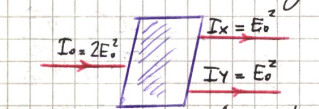
\includegraphics[width=0.4\textwidth]{images/fig_ft2_birref.jpg}

se tienen dos estados. Este sistema es similar a lo que se vio previamente. A la salida tengo
dos estados.
Lo que entrará será 
\[
	\vb E = E_0 ( \xver + \yver ) \euler^{i( kz - \omega t)}
\]
y la analogía me lleva a que polarización de luz en $\xver$ y $\yver$ equivalen a $S_z^+$ y $S_z^-$,
respectivamente.
Repetimos los experimentos, pero ahora con luz.

Matemáticamente el filtro en $\xver$ es un ente que lo que hace es proyectar la luz entrante
en $\xver$.

Los tres casos entonces corresponden a:

{\bf 1}

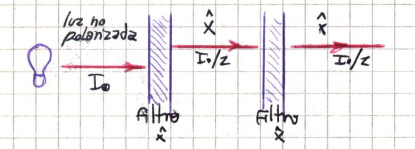
\includegraphics[width=0.5\textwidth]{images/fig_ft2_polarizacion_1.jpg}

No hay efecto neto. Opera como un filtro en $\xver$ del modo $(\vb E\cdot\xver)\xver$
y lo que sale es $E_0 \xver \euler^{i( kz - \omega t)}$

{\bf 2}

En este caso el filtro a $\pi/4$ lo que hace es proyectar en $\xver', \yver'$

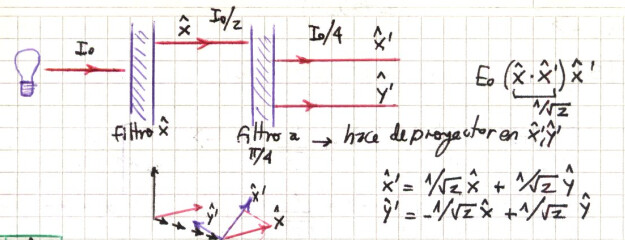
\includegraphics[width=0.5\textwidth]{images/fig_ft2_polarizacion_2.jpg}

Se tienen a la salida $E_0(\xver\cdot\xver')\xver$ donde
\[
	\xver' = \frac{1}{\sqrt{2}} \xver +  \frac{1}{\sqrt{2}} \yver \qquad \qquad 
	\yver' = -\frac{1}{\sqrt{2}} \xver +  \frac{1}{\sqrt{2}}, 
\]
de manera que $S_x^+$ equivale a $\xver'$ y $S_x^i$ equivale a $\yver'$.

{\bf 3}

Aquí se ve que filtrar dos veces es incompatible con el electromagnetismo.
A la salida se tiene $E_0(\xver'\cdot\xver)\xver$, de modo que aparece una componente
que no estaba presente.

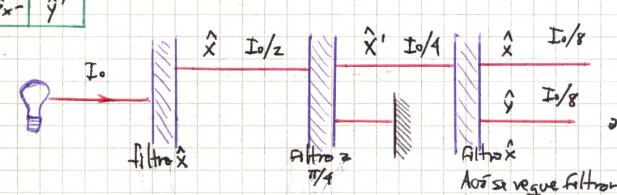
\includegraphics[width=0.5\textwidth]{images/fig_ft2_polarizacion_3.jpg}

Entonces
\[
	\vb E = E_0 \left( 
	\frac{1}{\sqrt{2}} \: \xver \cos( (kz-\omega t) ) + \frac{1}{\sqrt{2}} \: \yver \cos( (kz-\omega t) )
	\right) =
	E_0 \left( \frac{ \xver \pm i \yver }{\sqrt{2}} \right) \euler^{i(kz-\omega t)}
\]
de manera que con un cristal birrefringente que separe izquierda-derecha en luz polarizada
circular puedeo continuar la equivalencia
$S_y^+ \equiv \text{right}$ y $S_y^- \equiv \text{left}$ y tenemos seis estados pero son
solo dos los independientes.

Hacen falta vectores complejos para describir sistemas cuánticos. Ya en este sencillo caso
de analogía luz-spin vemos que la descripción completa del problema no puede hacerse en
términos de vectores con coeficientes reales.
Necesitamos un espacio complejo.

El problema del spin es sencillo porque es discreto y de dos estados.

La amplitud de probabilidad será algo como
\[
	A \sim \hat{i} \cdot \hat{j}
\]
donde j es el filtro. Luetgo la probabilidad es
\[
	P = |A|^2 = (\hat{i} \cdot \hat{j})(\hat{i} \cdot \hat{j})^*.
\]
Para operar construiremos un formalismo.

\subsection{El formalismos}

El formalismo para la mecánica cuántica incluirá
\begin{itemize}
	\item Estados
	\item Productos entre estados (propiedades matemáticas)
	\item Operadores, que llevan a observables
	\item Postulados de la mecánica cuántica
\end{itemize}

Para el caso del spin se definen
\[	
	S =\frac{1}{2} \qquad \qquad S_z^+, S_z^-
\]
y se definen los kets $\Ket{ \: }$ que tendrán toda la información. Inventados por P.A.M. Dirac.
No son otra cosa que vectores con coeficientes complejos.
La base de polarización (estados) será
\[
	\Ket{S_z;+} \qquad \qquad \Ket{S_z;-}
\]
y entonces $\Ket{S_x;+}$ es una combinación lineal de 1,2 anteriores.
Así
\[
\begin{array}{rr}
	\Ket{S_x;+} &= \displaystyle \frac{1}{\sqrt{2}} \Ket{S_z;+} + \frac{1}{\sqrt{2}} \Ket{S_z;+} \\
	& \\
	\Ket{S_x;-} &=\displaystyle  -\frac{1}{\sqrt{2}} \Ket{S_z;+} + \frac{1}{\sqrt{2}} \Ket{S_z;-} \\
	& \\
	\Ket{S_y;+} &=\displaystyle  \frac{1}{\sqrt{2}} \Ket{S_z;+} + \frac{i}{\sqrt{2}} \Ket{S_z;-} \\
	& \\
	\Ket{S_y;-} &=\displaystyle  \frac{1}{\sqrt{2}} \Ket{S_z;+} - \frac{i}{\sqrt{2}} \Ket{S_z;-}
\end{array}
\]
aunque probar esto no es ninguna boludez.


% =================================================================================================
\section{Algebra?}
% =================================================================================================

El ket contiene toda la información cuántica del estado. Da el estado físico del sistema.
Cumplen las siguientes propiedades
\begin{itemize}
	\item $\Ket{\alpha} + \Ket{\beta}$ la suma de kets es un ket
	\item $c\Ket{\alpha}= \Ket{\alpha} c$ con $c\in\mathbb{C}$
	\item $c_1\Ket{\alpha} + c_2\Ket{\beta} = \Ket{\gamma}$ con $c_1,c_2 \in \mathbb{C}$
	\item $c\Ket{\alpha},\Ket{\alpha}$ representan el mismo estado cuántico
\end{itemize}

Se define un espacio de {\it Bra} dual al de "kets" al que se va mediante ``dual conjugado''
\[
	\Ket{a}, \Ket{a'} \Leftrightarrow \Bra{a}, \Bra{a'}
\]
\[
	\Ket{a} + \Ket{b} \leftrightarrow \Bra{a} + \Bra{b} \qquad 
	c\Ket{a} \leftrightarrow c^*\Bra{a}
\]
\[
	c_a \Ket{a} + c_b \Ket{b} \leftrightarrow c_a^* \Bra{a} + c_b^*\Bra{b}
\]

Se define también un producto interno según
\[
	(\Bra{\alpha})(\Ket{\beta}) \equiv \Braket{\alpha|\beta}
\]
que no es otra cosa que un número complejo. Se puede hacer entonces una equivalencia con los vectores
estándard del álgebra del siguiente modo 
\[
	\text{ket} \sim \text{vector columna} \qquad \Ket{x} = \begin{pmatrix}
	                                                       1 \\
	                                                       0 \\
	                                                      \end{pmatrix}
\]
\[
	\text{bra} \sim \text{vector fila} \qquad \Bra{x} = ( 1 \; 0 )          
\]
y habiendo definido esta base escribimos, por ejemplo
\[
	\Ket{a} = \frac{1}{\sqrt{2}} \begin{pmatrix} 1 \\ 1  \\ \end{pmatrix}  =
	\frac{1}{\sqrt{2}} \begin{pmatrix} 1 \\ 0  \\ \end{pmatrix}  + 
	\frac{1}{\sqrt{2}} \begin{pmatrix} 0 \\ 1  \\ \end{pmatrix} =
	\frac{1}{\sqrt{2}} \Ket{x} + \frac{1}{\sqrt{2}} \Ket{y} 
\]
\[
	\Braket{a|x} = \frac{1}{\sqrt{2}}( 1 \; 1)\begin{pmatrix} 1 \\ 0  \\ \end{pmatrix} = \frac{1}{\sqrt{2}}
\]
y del mismo modo
\[
	\left( \frac{1}{\sqrt{2}} \Bra{x} + \frac{1}{\sqrt{2}} \Bra{y}  \right)
	\left( \Ket{x} \right)= \frac{1}{\sqrt{2}}.
\]
La trasposición opera como en álgebra, transmutando de ket a bra y viceversa.
\[
	\xver' = \frac{1}{\sqrt{2}}\begin{pmatrix}
	                            1 \\
	                            0 \\
	                           \end{pmatrix}
	                           \qquad \qquad 
	(\xver')^\dagger = \frac{1}{\sqrt{2}} (1 \; 0) 
\]

El producto interno tiene las siguientes propiedades:
\begin{enumerate}
	\item $\Braket{\beta|\alpha} = \Braket{\beta|\alpha}^*$ \text{luego} $ \Braket{\alpha|\alpha} \; \in \mathbb{R}$
	\item $\Braket{\alpha|\alpha} \geq 0$ \text{métrica definida positiva}
	\item $\Braket{\alpha|\beta} = \Braket{\beta|\alpha} = 0 \Leftrightarrow \Ket{\alpha} \perp \Ket{\beta}$
	\item $\Braket{\tilde{\alpha}|\tilde{\alpha}} = 1 \; \text{con} \; 
	\Ket{\tilde{\alpha}} = \frac{1}{\sqrt{\Braket{\alpha|\alpha}}}\Ket{\alpha} $ todo ket no nulo es normalizable
\end{enumerate}

La primera propiedad busca que podamos darle significado probabilístico.
El producto $\Braket{\a|\a}$ da la norma al cuadrado.

\begin{ejemplo}{\bf Veamos que el estado de spin $S_x^+$ está normalizado}

Para ello escribimos su expresión en términos de los estados $S_z$ y aplicamos dual conjugado.
Luego, 
\[
	\Braket{ S_x ; + | S_x ; + } =
	\left( \frac{1}{\sqrt{2}} \Bra{S_z;+} + \frac{1}{\sqrt{2}} \Bra{S_z;-} \right) 
	\left( \frac{1}{\sqrt{2}} \Ket{S_z;+} + \frac{1}{\sqrt{2}} \Ket{S_z;-} \right) 
\]
\[
	\Braket{S_x,+|S_x,+} =  \frac{1}{\sqrt{2}} \Braket{S_z;+|S_z;+} +
	\frac{1}{\sqrt{2}} \Braket{S_z;+|S_z;-} +
	\frac{1}{\sqrt{2}} \Braket{S_z;-|S_z;+} +
	\frac{1}{\sqrt{2}} \Braket{S_z;-|S_z;-} = 1
\]

\end{ejemplo}

Recordemos que en la formulación de mecánica cuántica que se utilizó en anteriores cursos, F4,
se tenían funciones de onda que se pueden ver como una notación relacionada con kets y bras
a través del producto interno.
\[
	\Braket{ \b | \a } = \int d^3x \: \phi^*_\b(\vbx) \: \phi_\a(\vbx) 
\]


\subsection{Operadores}

A cada observable lo representaremos por un operador. Hay operaradores que no vienen de observables.
\[
	\hat{A}\Ket{\alpha} = \Ket{\gamma} \qquad \qquad  \Bra{\alpha} \hat{A} = \Bra{\gamma}
\]
un operador sobre un ket da otro ket y sobre un bra da otro bra. Notemos que en este último caso opera 
a izquierda. Por el momento se trabajará con operadores lineales.

La transformación entre operadores se da con 
\[
	\hat{X}\Ket{a} \Leftrightarrow \Bra{a}\hat{X}^\dagger
\]
donde $\dagger$ (daga) significa el traspuesto conjugado; cambia el sentido hacia donde actúa el operador 
y conjuga. Se da que si 
\[
	\hat{X} = \hat{X}^\dagger \quad \Rightarrow \qquad \hat{X} \;\text{es hermítico}
\]
En mecánica cuántica todos los observables serán representados por operadores hermíticos.

Se dan 
\begin{itemize}
	\item $\hat{X}\hat{Y} \neq \hat{Y}\hat{X} \qquad \qquad \text{no conmutativo}$
	\item $\hat{X}(\hat{Y}\hat{Z}) = (\hat{X}\hat{Y})\hat{Z} = \hat{X}\hat{Y}\hat{Z} \qquad \qquad \text{asociativo}$
	\item $(XY)^\dagger = Y^\dagger X^\dagger$
	\item $\hat{0}\Ket{\alpha} = 0 \qquad \forall \Ket{\alpha}$ ; $\hat{0} \equiv$ operador nulo
	\item $\hat{X}( c_1 \Ket{\alpha} + c_2 \Ket{\beta} ) = c_1 \hat{X}\Ket{\alpha} + c_2 \hat{X}\Ket{\beta} $
\end{itemize}
de modo que en cuántica los observables se representan mediante operadores hermíticos.

\subsection{Sandwichs}

Coloquialmente encerrar un operador operando sobre un ket (bra) con un bra (ket).
Se obtiene un escalar
\[
	\Braket{\beta|X|\alpha} = (\Bra{\beta})(X\Ket{\alpha}) = \Braket{\beta|\gamma} =
	\Braket{\gamma|\beta}^* = (\Braket{\alpha|X|\beta})^*
\]
donde usamos que $\Ket{\gamma}$ es un ket y por dual conjugado $\Bra{\gamma} = \Bra{\alpha}\hat{X}^\dagger$ y
extraemos como conclusión 
\[
	\Braket{\beta|X|\alpha} = (\Braket{\alpha|X|\beta})^*,
\]
y de manera equivalente
\[
	\Braket{\beta|X|\alpha} = (\Bra{\beta}X^\dagger)(\Ket{\alpha}) = \Braket{\Gamma|\alpha} =
	\Braket{\alpha|\Gamma}^* = (\Braket{\alpha|X^\dagger|\beta})^*
\]
donde usamos que $\Bra{\Gamma}$ es un bra y por dual conjugado $\Ket{\Gamma} = \hat{X}\Ket{\beta}$.
El formalismo parece ser consistente. El operador opera sobre un ket/bra y multiplica al otro.

\notamargen{Las mediciones se pensarán como proyectar sobre autoestados.}

\subsection{Producto externo}

Es un nuevo tipo de producto entre vectores.
\[
	\Ket{\beta} \Bra{\alpha} \equiv (\Ket{\beta} )( \Bra{\alpha} )
\]
\[
	( \Ket{\beta} \Bra{\alpha} )\Ket{\gamma} = 
	\Ket{\beta} \Bra{\alpha} \Ket{\gamma} =
	\Braket{\alpha|\gamma} \Ket{\beta} , 
\]
de modo que es un operador pues al aplicar sobre un ket obtengo otro ket 
(notemos que $\Braket{\alpha|\gamma}$ es un escalar). Podemos pensar que 
\[
	\Lambda_\alpha \equiv \Ket{\alpha}\Bra{\alpha}
\]
es un nuevo operador, el proyector, que actúa rotando un $\Ket{\gamma}$ en 
la dirección de $\Ket{\beta}$. 
Notemos 
\[
	\Lambda_\alpha^2 = \Ket{\alpha}\Bra{\alpha}\Ket{\alpha}\Bra{\alpha} = 
	\Ket{\alpha}\Bra{\alpha} = \Lambda_\alpha
\]
puesto que $\Braket{\alpha|\alpha}=1$, de manera que aplicar dos veces un 
proyector no cambia nada.
El proyector $\Lambda_\alpha$ sobre un ket $\Ket{\beta}$ selecciona la parte de
$\Ket{\beta}$ en la dirección de $\Ket{\alpha}$. Nos dice cuanto de $\Ket{\beta}$ 
está en la dirección de $\Ket{\alpha}$.
Luego,
\[
	\sum_i^N \; \Lambda_i = \sum_i^N \; \Ket{i}\Bra{i} = \mathbb{1}
\]
la suma de todos los proyectores del espacio en el que estamos es la identidad de
ese espacio.
Decimos que $\{ \Ket{i} \}$ es un conjunto completo. 

\begin{ejemplo}{\bf Traspuesto de un producto externo}

Queremos ver que si $X = \Ket{\beta} \Bra{\alpha}$, entonces $X^\dagger = \Ket{\alpha} \Bra{\beta}$.
Hacemos operar sobre estados arbitrarios, y sabiendo que valen 
\[
	\Braket{a|X|b} = \Braket{b|X^\dagger|a}^* \qquad \qquad \Braket{a|X|b}^* = \Braket{b|X^\dagger|a}
\]
se tiene, reemplazando la definición de $X$,
\[
	 \Braket{a|(\Ket{\beta} \Bra{\alpha})|b}^* = \Braket{b|(\Ket{\beta} \Bra{\alpha})^\dagger|a}
\]
\[
	 \Braket{a|\beta}^* \Braket{\alpha|b}^* = \Braket{\beta|a} \Braket{b|\alpha} =
	 \Braket{b|\alpha}\Braket{\beta|a} = \Braket{b|(\Ket{\beta} \Bra{\alpha})|a}
\]
y comparando este último resultado con el de la línea anterior, vemos que se verifica
\[
	\Ket{\a} \Bra{\b} = (\Ket{\beta} \Bra{\alpha})^\dagger.
\]
 
\end{ejemplo}

\begin{ejemplo}{\bf Ejemplo sencillo 2D}
 
Consideramos versores en el plano, vectores columna,
\[
	\hat{X} = \begin{pmatrix} 1 \\ 0 \end{pmatrix} \qquad \qquad \hat{Y} = 
	\begin{pmatrix} 0 \\ 1 \end{pmatrix}
\]
que en sus versiones dagueadas pasan a ser vectores fila
\[
	\hat{X}^\dagger = ( 1 \; 0 ) \qquad \qquad \hat{Y}^\dagger = ( 0 \; 1  ) 
\]

Luego, los productos que podemos hacer corresponden a las operaciones matriciales de
vector por vector, resultando en número o matriz dependiendo del orden
\[
	\hat{X}^\dagger\hat{X} = (1 \; 0) \begin{pmatrix} 1 \\ 0 \end{pmatrix} = 1 \qquad 
	\hat{X}\hat{X}^\dagger = \begin{pmatrix} 1 \\ 0 \end{pmatrix} (1 \; 0) = 
	\begin{pmatrix} 1 & 0 \\ 0 & 0 \\ \end{pmatrix},
\]
donde instamos al lector a que note la diferencia de dimensión en los resultados.
En la notación de Dirac estos versores serían $\Ket{x}, \Ket{y}$ y sus correspondientes
bras. Luego,
\[
	\Braket{x|x} = \Braket{y|y} = 1, \qquad \qquad \Braket{x|y} = \Braket{y|x} = 0
\]
y las matrices serían los proyectores
\[
	P_x \equiv \Ket{x}\Bra{x}, \qquad \qquad  P_y \equiv \Ket{y}\Bra{y}.
\]

Para un estado arbitrario $\Ket{\a} = \a_x \Ket{x} + \a_y \Ket{y}$, si uso el proyector
$P_x$ se tendrá
\[
	P_x \Ket{\a} = (\Ket{x}\Bra{x})(\a_x \Ket{x} + \a_y \Ket{y})
\]
\[
	P_x \Ket{\a} = \a_x \Ket{x}\Braket{x | x} + \a_y \Ket{x}\Braket{x |y} =
	\a_x \Ket{x}.
\]
Del mismo modo se obtiene $P_y \Ket{\a} = \a_y \Ket{y}$. Si sumo ambos proyectores obtengo
la identidad
\[
	(P_x + P_y)\Ket{\a} \equiv I \Ket{\a} = \Ket{\a},
\]
y vemos que la identidad no hace nada.

\end{ejemplo}

Los kets $\Ket{\alpha}$ {\it viven} en un espacio vectorial de Hilbert con dimensión $N$, donde
$N$ lo dicta el número de posibles estados de cada sistema físico. 
Una partícula de spín $1/2$ sólo tiene dos estados: up y down.

Hay otro producto más, entre dos bras o dos kets, que se llama producto tensorial y se representa 
como 
\[
	\Ket{\alpha} \otimes \Ket{\beta} \qquad \qquad \Bra{\alpha} \otimes \Bra{\beta}
\]
que es un producto entre kets de espacios de Hilbert diferentes; el resultado no es ni un bra ni
un ket. Digamos que es una notación.
\[
	\Braket{\alpha|\beta}^* \equiv DC\{\ket{\beta}\} DC\{\Bra{\alpha}\}
\]

\section{Bases}

Dado un sistema físico representado por un espacio vectorial $\mathcal{H}$ de dimensión $N$ existirá una base (también 
de dimensión $N$) que será un conjunto de estados tal que cualquier estado de ese sistema físico puede representarse 
como combinación lineal de ese conjunto,
\[
	\{ \Ket{i}\} \; \text{base} \quad \Rightarrow \; \Ket{\alpha} = \sum_i^N c_i \Ket{i}
\]
siendo $\Ket{\alpha}$ un estado cualquiera.
Es práctico utilizar bases ortonormales,
\[
	\Braket{ i|j } = \delta_{ij} = \begin{cases}
	                                1 \quad i=j \\
	                                0 \quad i\neq j
	                               \end{cases}
\]
que es la delta de Kronecker.

Así, los kets se definen normalizados, dado un ket
\[
	\Ket{\phi} =  a \Ket{1} + b \Ket{2} + c \Ket{3}
\]
se lo normaliza con
\[
	\Ket{\psi} = \frac{1}{\Braket{\phi|\phi}}\:\Ket{\phi}
\]
lo que significa que 
\[
	\Ket{\psi} = a' \Ket{1} + b' \Ket{2} + c' \Ket{3} \qquad\qquad |a'|^2 + |b'|^2 +|c'|^2 = 1
\]
Si tenemos un ket normalizados,  $\Ket{\phi} = a \Ket{1} + b \Ket{2}$ y su bra 
$\Bra{\phi} = a^*\Bra{1} + b^* \Bra{2}$, entonces 
\begin{multline*}
 	\Braket{\phi|\phi} = (a^*\Bra{1} + b^* \Bra{2})(a \Ket{1} + b \Ket{2}) = \\
	a^*a \Braket{1|1} + b^*a\Braket{2|1} + a^*b\Braket{1|2} + b^*b\Braket{2|2} =
	|a|^2 + |b|^2 = 1
\end{multline*}
	

\subsection{Autokets y autovalores}

Si $\hat{A}\Ket{a}=c\Ket{a}$ entonces $\Ket{a}$ es autoket de $\hat{A}$ con autovalor $c$. Se suelen 
etiquetar los autoestados $\Ket{a'}, \Ket{a''}$ de modo que 
\[
	\hat{A}\Ket{a'} = a'\Ket{a'}
\]
lo cual lleva al problema espectral
\[
	\left(\hat{A} - a'\mathbb{1}\right) \Ket{a'} = 0
\]
entonces los operadores tendrán representación matricial, que cambiará según la base utilizada.
Vamos viendo que en general sólo se sabe cómo opera un operador sobre kets. La operación sobre los
bras la obtenemos usando dual conjugado.

Lo siguiente debiera ser amparado por un título como ``propiedades de operadores hermíticos''.

Deducimos entonces que
\begin{enumerate}
	\item Los autovalores de un operador hermítico son reales y los autokets correspondientes a diferentes
	autovalores son ortogonales.
	\item Los autokets de un operador son base completa del espacio de kets.
\end{enumerate}

Como ejemplo de A citemos
\[
	A\Ket{a'} = a' \Ket{a'} \quad \text{DC} \quad \Bra{a'} A^{\dagger} = \Bra{a'} A = \Bra{a'}a'^*
\]
de manera que 
\[
	\Braket{a'|A|a'} = \Bra{a'} ( A\Ket{a'} ) = a'
\]
\[
	( \Braket{a'|A|a'} )^* = ( \Bra{a'} )( A\Ket{|a'} )^* = ( \Bra{|a'}A^\dagger )( \Ket{a'} )
\]
\[
	= \Braket{a'|A|a'} = a' \qquad \Rightarrow \quad a' = a'^*.
\]
Me gusta más la otra forma, que es meter otro $a''$ así
\[
	\Braket{a''|A|a'} = a' \Braket{a''|a'} \qquad \qquad \Braket{a''|A^\dagger|a'} = a''^* \Braket{a''|a'}
\]
de manera que como
\[
	(a' - a''^*) \Braket{a''|a'} = 0,
\]
si $\Ket{a'}=\Ket{a}$ entonces $a' = a'^*$ y los autovalores son reales. En cambio si $\Ket{a'}\neq\Ket{a''}$ 
se tiene $a'\neq a''$ entonces  $\Braket{a''|a'} = 0$ y los autoestados del operador son perpendiculares.
Ya está abajo esto.

Para el caso de B se postula así. Si esto vale entonces 
\[
	\Ket{\alpha} = \sum_i^N \Ket{a_i}\Bra{a_i} \Ket{\alpha} = \sum_i^N c_i \Ket{a_i} = 
	\mathbb{1}\Ket{\alpha}
\]
pues 
\[
	\Braket{\alpha|\alpha} = \sum_{i,j}^N \Braket{ a_j|c_j^* c_i|a_i} = \sum_i^N |c_i|^2 = 1
\]
y además 
\[
	A\Ket{a'} = a'\Ket{a'} \qquad A\Ket{a''} = a''\Ket{a''} \Rightarrow 
	A(\Ket{a'} - \Ket{a''} ) = a'\Ket{a'} - a''\Ket{a''}
\]
\[
	\Braket{ a''|A|a' } = a' \Braket{ a''|a' } \qquad \Braket{ a'|A|a'' } = a'' \Braket{ a'|a'' }
\]
y ahora conjugando
\[
	\Braket{ a''|A|a' }^* = a' \Braket{ a''|a' }^* \qquad \Braket{ a''|A|a' } = a'' \Braket{ a''|a' }
\]
donde usamos que $a''^* = a''$ y restando 
\[
	(a'-a'')\Braket{a''|a'} = 0 \qquad \Rightarrow \; \Braket{a''|a'} = 0 
		\quad \text{si} \quad a'\neq a''
\]
O sea, hemos probado que los autovectores correspondientes a diferentes autovalores son
ortogonales.


\subsection{Combinación lineal de autoestados}

Podemos escribir 
\[
	\Braket{a''|a'} = \delta_{a'a''}
\]
que es la delta de Kronecker.
Postulo que forman una base completa, y que un estado $\Ket{\alpha}$ se puede escribir en 
función de la base $\Ket{a_i}$ de esta forma 
\[
	\Ket{\a} = \sum_{a'}  C_{a'} \Ket{a'}.
\]

Ahora quisiéramos ver quién es el coeficiente $C_{a'}$.
Para ello multiplicamos por un bra arbitrario
\[
	\Braket{a_j|\alpha} = \sum_{i=1}^N C_i \underbrace{\Braket{a_j|a_i}}_{\delta_{ij}} = C_j, 
\]
de modo que es
\[
	\Ket{\alpha} = \sum_{i=1}^N \Ket{a_i}\Braket{a_i|\alpha} = 
		\sum_{i=1}^N \Braket{a_i|\alpha} \: \Ket{a_i}
\]
o bien, en términos del operador $\Lambda$ [?],
\[
	\Ket{\alpha} = \left( \sum_{i=1}^N \Ket{a_i}\Bra{a_i} \right) \Ket{\alpha} 
\]
de modo que si la base es completa debe ser
\[
	\sum_{i=1}^N \Ket{a_i}\Bra{a_i} \equiv \mathbb{1}.
\]

Todos estos resultados surgen de suponer que los autoestados son una base completa.
Es análogo a la proyección de un vector en un sistema coordenado: 
$\vb V = \sum_i (\vb V\cdot \hat{e}_i ) \hat{e}_i $.

Asimismo, considerando la normalización de estados
\[
	\Braket{\a|\a} = 1 =
	\Bra{\a} \sum_{a'}\Ket{a'} \Braket{a'|\a} = \sum_{a'} \Braket{\a|a'} \Braket{a'|\a}
\]
o bien
\[
	\Braket{\a|\a} = 1 = \sum_{a'} C_{a'}^* C_{a'} = \sum_{a'} |C_{a'}|^2.
\]

% Si la base es completa entonces es $\sum \Lambda = 1$.

\subsection{Operadores y matrices}

Un operador se puede representar matricialmente como 
\[
	X = \sum_{a'}^N  \sum_{a''}^N \Ket{a''} \Bra{a''} X \Ket{a'} \Bra{a'} =  
	\sum_{a'}^N  \sum_{a''}^N ( \Braket{a''|X|a'} ) \Ket{a''} \Bra{a'}
\]
donde hemos explotado el hecho de que en el medio aparece un escalar (?), siendo 
\[
	X_{ij} = \Braket{a_i|X|a_j}
\]
un elemento de matriz. Y notemos que $\Ket{a''} \Bra{a'}$ es un ente de $N\times N$.
Si la base es de dimensión 3 se tendrá por ejemplo,
\[
	X = \begin{pmatrix}
	 x_{11} & x_{12} & x_{13} \\
	 x_{21} & x_{22} & x_{23} \\
	 x_{31} & x_{32} & x_{33} \\
	\end{pmatrix}
\]
de manera que existe una identificación entre cosas del álgebra básica y este mundo
de operadores y estados.
Si $X$ es hermítico por ejemplo, entonces su matriz es simétrica conjugada.
\[
	\Braket{a_i|X|a_j}^* = (\Bra{a_j}X^\dagger)(\Ket{a_i}) = \Braket{a_j|X|a_i}
\]
y entonces 
\[
	\Braket{a_j|X|a_i}^* = \Braket{a_i|X|a_j}
\]
de modo que 
\[
	X_{ji}^* = X_{ij} \qquad X_{ij}^{t*} = X_{ij} \qquad X_{ij}^\dagger=X_{ij}
\]
y vemos bien el significado de {\it daguear}. En este caso la matriz tiene traza real
y seis elementos independientes
\[
	X = \begin{pmatrix}
	  X_{11} & X_{12} & X_{13} \\
	  X_{12}^* & X_{22} & X_{23} \\
	  X_{13}^* & X_{23}^* & X_{33} \\
	\end{pmatrix} =
	\begin{pmatrix}
	  X_{11} & X_{12} & X_{13} \\
	  X_{21} & X_{22} & X_{23} \\
	  X_{31} & X_{32} & X_{33} \\
	\end{pmatrix} =
	\begin{pmatrix}
	  X_{11}^* & X_{21}^* & X_{31}^* \\
	  X_{12}^* & X_{22}^* & X_{32}^* \\
	  X_{13}^* & X_{12}^* & X_{33}^* \\
	\end{pmatrix}
\]

La traza será
\[
	\text{ tr }(A) = \sum_{i=1}^N \Braket{ a_i | A | a_i }.
\]


\subsection{Cambio de base}

Para cambiar de base metemos un uno ($\mathbb{1}$) escrito como suma de proyectores,
\[
	X\Ket{b_j} = \mathbb{1} \: X\Ket{b_j} = \sum_{i=1}^N \Ket{a_i}\Braket{a_i|X|b_j} = 
	\sum_{i=1}^N C_{ij} \Ket{a_i}
\]
siendo $C_{ij}$ la matriz del cambio de base.
Se puede escribir
\[
	\Ket{b_j} = \sum_{i=1}^N \Ket{a_i}\Braket{a_i|b_j} 
\]
y se ve que $\Braket{a_i|b_j}$ son los elementos de la matriz que cambia de base.

\begin{ejemplo}{\bf Ejercicio 2}

Tenemos la base $\{ \Ket{+}, \Ket{-} \}$, o sea un espacio de Hilbert de dimensión 2. Se considera
ortonormal de manera que
\[
	\Braket{+|+} = \Braket{-|-} = 1 \qquad \Braket{+|-} = 0
\]
Luego, se tiene
\[
	S_x = \frac{\hbar}{2} (\: \Ket{+}\Bra{-} + \Ket{-}\Bra{+} \:)
\]
Los elementos de matriz serán
\[
	(S_x)_{11} = \Bra{+} (S_x ) \Ket{+} =
	 \frac{\hbar}{2} \Bra{+} (\: \Ket{+}\Bra{-} + \Ket{-}\Bra{+} \:) \Ket{+} = 0,
\]
dado que ambos miembros dan $\Braket{+|-}$. Asimismo,
\[
	S_x \Ket{+} = \frac{\hbar}{2} ( \Ket{+}\Bra{-} + \Ket{-}\Bra{+} ) \Ket{+} = \frac{\hbar}{2}\Ket{-}
\]
y 
\[
	S_x \Ket{-} = \frac{\hbar}{2}\Ket{+}.
\]

Matricialmente
\[
	S_x = \frac{\hbar}{2} \: \begin{pmatrix}
	0  &  1 \\
	1  &  0
	\end{pmatrix}
\]
de manera que
\[
	S_x \Ket{+} = \frac{\hbar}{2} \: \begin{pmatrix}
	0  &  1 \\
	1  &  0
	\end{pmatrix}
	\begin{pmatrix}
	 1 \\
	 0
	\end{pmatrix}
	=
	\frac{\hbar}{2} \: 
	\begin{pmatrix}
	 0 \\
	 1
	\end{pmatrix}.
\]
 
\end{ejemplo}

\begin{ejemplo}{\bf Ejercicio 6}
 
Tenemos un espacio de kets generado por $\{ \Ket{a'} \}$ ortogonales, siendo $A$ hermítico, de
manera que los $a$ son reales.

i) Queremos probar que $\Pi_{a'} (A - a'\mathbb{1})$ es el operador nulo. Luego, supongamos que 
\[
	\Pi_{a'} (A-a'\mathbb{1}) \equiv O
\]
y entonces verificará
\[
	\Braket{a'|O|a''} = O_{a'a''} = 0.
\]
Tomemos
\[
	\Pi_{a'} (A-a'\mathbb{1}) \Ket{a''} = \Pi_{a'} A \Ket{a''} - a\mathbb{1} \Ket{a''}
	= \Pi_{a'} (\Ket{a''} + a' ) \Ket{a''}
\]
pero lo que opera sobre el ket es nulo.

Por otra parte, como $(A-a_n\mathbb{1})\Ket{a''}$ se puede escribir
\[
	(A-a_{n_2}\mathbb{1})(A-a_{n_1}\mathbb{1})\Ket{a''}( a'' - a_n )
\]
y sigue pasadno de modo que al final se obtiene
\[
	\Ket{a''} \Pi_{a'} (a'' - a').
\]

ii) Y ahora, qué significa el siguiente operador
\[
	\Pi_{a' \neq a''} \frac{ (A-a''\mathbb{1}) }{ ( a' - a'' ) }
\]
Aplicamos a un ket $\Ket{a}$,
\[
	\Pi_{a' \neq a''} \frac{ (A-a''\mathbb{1}) }{ ( a' - a'' ) } \Ket{a} = 
	\Pi_{a' \neq a''} \frac{ ( a - a'' ) }{ ( a' - a'' ) } \Ket{a}
\]
y será nulo sí y sólo si $a \neq a''$, de manera que es una construcción de la delta de Kronecker,
\[
	\Pi_{a' \neq a''} \frac{ (A-a''\mathbb{1}) }{ ( a' - a'' ) } = \delta_{aa'}\Ket{a'}
\]
Es un proyector de todos los elementos en $\Ket{a'}$ lo que siempre da cero para los de la base
salvo cuando es $a'=a$.
 
\end{ejemplo}

\begin{ejemplo}{\bf Ejercicio 8}

Consideramos $\vb S\cdot \nver$ donde $\vb S = ( S_x, S_y, S_z )$ o sea un vector de operadores y el
versor es el usual de esféricas en términos de los ángulos.
\[
	\nver = (\sin\b\cos\a, \sin\b\sin\a, \cos\b).
\]
\end{ejemplo}

\begin{ejemplo}{\bf Ejercicio 11}
 
Consideremos la matriz $M$ hermítica y la base $\{ \Ket{1}, \Ket{2}, \Ket{3} \}$ que tendrá por ello
autovalores relaes y autovectores ortogonales.
\[
	M = \begin{pmatrix}
	     0 & 1 & 0 \\
	     1 & 0 & 1 \\
	     0 & 1 & 0 
	    \end{pmatrix}
\]
Los autovalores saldrán de
\[
	\left| \frac{1}{\sqrt{2}} \begin{pmatrix}
	                         -\lambda & 1 & 0 \\  
	                         1 & -\lambda & 1 \\
	                         0 & 1 & -\lambda 
	                          \end{pmatrix}
				\right| = -\lambda(\lambda^2 -1) = 0
\]
que dará $\lambda = 0,1,-1$.
Los autovectores salen de resolver 
\[
	\begin{pmatrix}
	0 & 1/\sqrt{2} & 0 \\
	1/\sqrt{2} & 0 & 1/\sqrt{2} \\
	0 & 1/\sqrt{2} & 0 
	\end{pmatrix}
	\begin{pmatrix}
	v_1^{(1)} \\
	v_2^{(1)} \\
	v_3^{(1)}
	\end{pmatrix} = 0
\]
y haciendo $v_2^{(1)} =0$ se tiene $v_1^{(1)} =-v_3^{(1)} $ y luego
\[
	v^{(1)}  =\frac{1}{\sqrt{2}} \begin{pmatrix}
	                              1 \\
	                              0 \\
	                              -1
	                             \end{pmatrix}
\]
con $\Braket{v^{(1)}|v^{(1)}} =1$ y así siguiendo con los otros vectorcillos, resulta
\[
	A = \left[ v^{(1)} v^{(2)} v^{(3)} \right] = 
	\begin{pmatrix}
	    0 & 0 & 0 \\
	    0 & 1 & 0 \\
	    0 & 0 & -1 
	\end{pmatrix}
\]
 
\end{ejemplo}

\subsection{Representación diagonal}

Un operador tiene representación diagonal cuando está representado en la base de sus
autokets
\begin{multline*}
 	A = \sum_i^N\sum_j^N \Ket{a_i}\Braket{a_i|A|a_j}\Bra{a_j} =
		\sum_i^N\sum_j^N a_j\Ket{a_i}\Braket{a_i|a_j}\Bra{a_j} = \\
		\sum_{i,j}^N \delta_{ij} a_j \Ket{a_i}\Bra{a_j} = \sum_i^N a_i \mathbb{1}
\end{multline*}
% \[
% 	A = \sum_i^N\sum_j^N \Ket{a_i}\Braket{a_i|A|a_j}\Bra{a_j} =
% 		\sum_i^N\sum_j^N a_j\Ket{a_i}\Braket{a_i|a_j}\Bra{a_j} =
% 		\sum_{i,j}^N \delta_{ij} a_j \Ket{a_i}\Bra{a_j} = \sum_i^N a_i \mathbb{1}
% \]
\[
	A = \begin{pmatrix} 
		a_1 & 0 & ... & 0 \\
		0 & a_2 & ... & 0 \\
		0 & 0 & ... & 0 \\
		0 & 0 & ... & a_n \\
	\end{pmatrix}
\]
y $a_1,a_2,...,a_n$ son sus autovalores.
Es destacable que es conveniente utilizar como bases los autoestados de ciertos operadores.

\subsection{Representaciones canónicas}

Podemos representar una base como vectores canónicos
\[
	\Ket{a_1} = \begin{pmatrix}
			1 \\
			0 \\
			. \\
			. \\
			N
			\end{pmatrix} \qquad 
	\Ket{a_1} = \begin{pmatrix}
			0 \\
			1 \\
			. \\
			. \\
			N
			\end{pmatrix} \qquad 
	\Ket{a_n} = \begin{pmatrix}
			0 \\
			0 \\
			. \\
			. \\
			1
			\end{pmatrix}
\]
luego 
\[
	\Ket{\alpha} = \sum_i \Ket{a_i}\Braket{a_i|\alpha} =
		\Braket{a_1|\alpha} \begin{pmatrix}
			1 \\
			0 \\
			. \\
			. \\
			N
			\end{pmatrix} +
		\Braket{a_2|\alpha} \begin{pmatrix}
			0 \\
			1 \\
			. \\
			. \\
			N
			\end{pmatrix} +
			... +
		\Braket{a_n|\alpha} \begin{pmatrix}
			0 \\
			0 \\
			. \\
			. \\
			1
			\end{pmatrix} =
\]
\[
	\begin{pmatrix}
		\Braket{a_1|\alpha} \\
		\Braket{a_2|\alpha} \\
			... \\
			... \\
		\Braket{a_n|\alpha}
	\end{pmatrix}
\]
y por DC se tiene 
\[
	\Bra{\alpha} = ( \; \Braket{\alpha|a_1} \quad \Braket{\alpha|a_2} 
	\quad ... \quad \Braket{\alpha|a_n} \; )
\]
y 
\[
	\Braket{\alpha|\alpha} = 1 = \overbrace{( \phantom{1} \qquad \phantom{1} )}^{1\times 
N}\overbrace{\begin{pmatrix} \phantom{1} \\ 	\phantom{1}  \end{pmatrix} }^{N\times 1} = \Box
\]
que es un escalar.
El producto entre otros dos estados arbitrarios
\[
	\Braket{\beta|\alpha} = \Braket{\beta|a_i} \Braket{a_i|\alpha} = 
	\sum_i^N \Bra{\beta} \underbrace{\Ket{a_i} \Bra{a_i}}^{\Lambda_{a_i}} \Ket{\alpha} = \Box 
\]
otra vez un escalar.

Para un operador $X$ se tiene la siguiente representación
\[
	X = \sum_i^N \sum_j^N \Ket{a_i} \Braket{a_i|X|a_j} \Bra{a_j} =
		\sum_i^N \sum_j^N  \Braket{a_i|X|a_j} \Ket{a_i} \Bra{a_j}
\]
y esto último es una matriz. Aquí el $\hat{X}$ es una matriz y 
$\Braket{a_i|\hat{X}|a_j} \equiv X_{ij}$ son sus elementillos (escalares).
En conclusión,
\[
	X = \sum_i^N \sum_j^N X_{ij} \: \Ket{a_i} \Bra{a_j},
\]
donde 
\[
	\Ket{a_i} \Bra{a_j} = \begin{pmatrix}
	 0 \\
	 ... \\
	 1 \\
	 ... \\
	 0
	\end{pmatrix}
	(\: 0 .... 1 .... 0 \:).
\]

Para un operador que actúa sobre un estado, dando otro estado, se tiene
\[
	\Braket{a_i|\gamma} = \Braket{a_i|X|\alpha} = \sum_{a_j} \Braket{a_i|X|a_j}\Braket{a_j|\alpha}
\]
que es el producto de una matriz por un vector
\[
	\begin{pmatrix}
	 \Braket{a_1|\gamma} \\
	 ... \\
	 ... \\
	\end{pmatrix} = 
	\begin{pmatrix}
	 X_{11} & X_{12} & ...\\
	 X_{21} & X_{22} & ... \\
	 ... \\
	\end{pmatrix}
	\begin{pmatrix}
	 \Braket{a_1|\alpha} \\
	 ... \\
	 ... \\	 
	\end{pmatrix}
\]

Para el producto externo será
\[
	\Ket{\b}\Bra{\a} = \sum_{a',a''} \Ket{a''} \Braket{a''|\b} \Braket{\a|a'} \Bra{a'}
\]
y este producto de brakets es la versión matricial del operador
\[
	\begin{pmatrix}	
	\Braket{a_1|\b} \Braket{a_1|\a}^* & \Braket{a_1|\b} \Braket{a_2|\a}^* & ... \\
	\Braket{a_2|\b} \Braket{a_1|\a}^* & \Braket{a_2|\b} \Braket{a_2|\a}^* & ... \\
	... & ... & 
	\end{pmatrix}
\]

En la base en la cual un operador es diagonalizable resulta sencilla su matriz:
\[
	A = \sum_{a',a''}  \Ket{a''} \Braket{a''|A|a'} \Bra{a'} = 
	\sum_{a'}  a' \Ket{a'} \Bra{a'} = \sum_{a'}  a' \Lambda_{a'},
\]
en términos del proyector.

Los elementos usados en el formalismo (bras, kets, etc.) pueden pensarse como vectores (fila
o columna) y matrices.

\section{Sistemas de spín 1/2}

Hay dos estados posibles de spin $(\Ket{+}, \Ket{-})$ entonces dimensión del espacio vectorial es 2. De 
manera que 
\[
	\mathbb{1} = \Ket{+}\Bra{+} \; + \;  \Ket{-}\Bra{-}
\]
\[
	\Ket{S_z ; +} = \Ket{S_z = \hbar/2} \equiv \Bra{+} 
\]
\[
	\Ket{S_z ; -} = \Ket{S_z = -\hbar/2} \equiv \Bra{-}
\]
\notamargen{Acá hay que diseñar unos $+,-$ que habiten dentro de los brakets pues estos se ven feo.}

Tenemos operadores de subida y de bajada,
\[
	S_+ = \hbar \Ket{+}\Bra{-} \qquad S_- = \hbar \Ket{-}\Bra{+}
\]
que actúan subiendo el spin o dando el ket nulo,
\[
	S_+ = \hbar \begin{pmatrix} 1 \\ 0 \end{pmatrix} ( 0 \; 1 ) 
		= \hbar \begin{pmatrix}  0 & 1 \\ 0 & 0 \end{pmatrix}
\]
o bien bajando el spín o dando el ket nulo,
\[
	S_- =\hbar \hbar \begin{pmatrix} 0 \\ 1 \end{pmatrix} ( 1 \; 0 ) 
	 = \hbar \begin{pmatrix} 0 & 0 \\ 1 & 0 \end{pmatrix}
\]

\subsection{Cambio de base}

Dados dos conjuntos base ortonormales y completos existe un $\widehat{U}$ unitario tal que 
\[
	U^+U=UU^+=\mathbb{1} \qquad \Ket{b_i}=U\Ket{a_i}
\]

Este operador de cambio de base será 
\[
	U = \sum_\ell \Ket{b_\ell}\Bra{a_\ell}
\]
\[
	U\Ket{a_i} = \sum_\ell \Ket{b_\ell}\Braket{a_\ell|a_i} = \Ket{b_i}
\]
que tiene por función pasar 
\[
	\underbrace{\Ket{a_\ell}}_{\text{vieja base}} \longrightarrow \underbrace{\Ket{b_\ell}}_{\text{nueva base}}
\]
\[
	\Braket{b_k|\alpha} = \sum_\ell \Braket{b_k|a_\ell}  \Braket{a_\ell|\alpha}  =
	\sum_\ell \Braket{a_k|U^+|a_\ell}  \Braket{a_\ell|\alpha} = \Braket{a_k|U^+|\alpha} 
\]

Entonces
\[
	\Ket{\text{nueva base}} = U \Ket{\text{vieja base}}
\]
\[
	\Braket{b_i | x | b_j} = \sum_{\ell,m} \Braket{b_i|a_\ell}\Braket{a_\ell|x|a_m}\Braket{a_m|b_j }
\]
\[
	\Braket{b_i | x | b_j} = \sum_{\ell,m}\Braket{a_i|U^+|a_\ell}\Braket{a_\ell|x|a_m}\Braket{a_m|U|a_j}
\]
\[
	X_{\Ket{b}} = U^+ X_{\Ket{a}} U,
\]
que es una transformación de similaridad.

\subsection{Mediciones y probabilidades}

En mecánica cuántica medir es filtrar. La medición perturba al sistema. Se miden variables dinámicas asociadas a 
observables.
Como los autoestados de un observable $\hat{A}$ son una base completa $\{\Ket{a_i}\}$ entonces un sistema se hallará en 
una combinación lineal de autoestados de $\hat{A}$, o al menos eso puede pensarse.


\begin{tabular}{|c|c|c|}
\hline
antes de medir & & luego de medir \\
\hline 
sistema en CL
de autestados de $\hat{A}$ & Medición de $\hat{A}$ & Salta a un autoestado de $\hat{A}$ \\
\hline 
sistema en 
autoestado de $\hat{A}$  & & Continúa en autoestado de $\hat{A}$ \\
\hline
\end{tabular}

Puede verse pictóricamente la medición así:
\[
	\Ket{\alpha} \longrightarrow \Ket{a'}
\]
el proceso de medición hace saltar hacia $\Ket{a'}$ siendo el resultado de la medida el autovalor $a'$.
Luego,
\[
	\mathrm{Prob}_{\Ket{a'}} \equiv |\Braket{a'|\alpha}|^2
\]

Antes de medir no puedo saber a qué estado saltará y tampoco en qué estado se hallaba. Si $P=1$ se halla en
$\Ket{a'}$ antes de saltar, si $P=0$ no se halla en $\Ket{a'}$ antes de saltar.

\subsection{Valor de expectación}

\[
	\Braket{\widehat{A}} \equiv \Braket{\alpha|A|\alpha}
\]c
el valor de expectación siempre se refiere a un estado en particular.
\[
	\Braket{A} = \sum_{a',a''} \Braket{\alpha|a'}	\Braket{a'|A|a''} \Braket{a''|\alpha}
\]
\[
	\Braket{A} = \sum_{a',a''}  \Braket{\alpha|a'} a''\delta_{a'a''} \Braket{a''|\alpha} =
			\sum_{a''} a''|\Braket{\alpha|a''}|^2
\]
\[
	\Braket{A} = \sum_{a',a''} = a'' \text{Prob}_{\Ket{a''}}
\]
Esto último tiene el sentido de una especie de promedio ponderado.


\subsection{Conmutadores}

Se definen, el conmutador
\[
	[ A, B] \equiv AB - BA,
\]
y el anticonmutador
\[
	\{ A, B \} \equiv AB + BA,
\]
y se dice que dos observables conmutan si $[A,B]=0$. Se dice que son compatibles si $[A,B]=0$ y anticompatibles si se 
da la contrario, $[A,B]\neq 0$.

TEOREMA:

Sean dos observables compatibles y no degenerados, entonces los autoestados $\{ \Ket{a'}\}$ de $A$ lo son también de 
$B$. Es decir que A y B tienen base de autoestados en común.

demostración:
\[
	\Braket{a'|AB-BA|a''} = 0 
\]
\[
	a' \Braket{a'|B|a''} - \Braket{a'|B|a''} a''= (a'-a'') \Braket{a'|B|a''}= 0 
\]
entonces 
\[
	\Braket{a'|B|a''} = 0
\]
y $B$ es diagonal en $\{ \Ket{a'}\}$.

Los autoestados son iguales pero no los autovalores; con lo cual se utilizará la notación $\Ket{a',b'}$ donde 
\[
	A \Ket{a',b'} = a' \Ket{a',b'} \qquad \qquad B \Ket{a',b'} = b' \Ket{a',b'}
\]

\subsection{Degeneración}

Puede darse que haya varios $g$ autoestados correspondientes a un mismo autovalor $a'$; entonces se dice que hay 
degeneración de orden $g$ para el autoestado $\Ket{a'}$
\[
	A\Ket{a'}= a'\Ket{a'} \quad ; i=1,2,...,g
\]
y $A$ tendrá una matriz de $m\times n$ bloques. 
En este caso no se puede decir que la base de $A$ diagonalice a $B$.\notamargen{Mejorar la matriz que está un asco}
\[
	A = \begin{pmatrix}
	     a'\mathbb{1} & 0 & & \\
	     0 & a''\mathbb{1} & & \\
	     & & a'''& \\
	     & & & a^IV \\
	     ...
	    \end{pmatrix}
\]
Los $\ket{a'_i}$ no dan información sobre los bloques correspondientes en la matriz de $B$.
Necesito un conjunto de operadores que haga romper la degeneración para expresar unívocamente 
el estado del sistema. Se llama CCOC. Necesito que conmuten entre sí para que las mediciones tengan sentido.

Si no conmutan entonces son incompatibles; la medición de uno hace saltar al sistema a un autoestado del otro y como no 
son comunes pierde sentido el concepto de medir. No tiene sentido la medición de algo si por el hecho de medir 
cambiamos lo que queremos medir.
Al ser incompatibles sus mediciones de afectan mutuamente.

Los autovalores de algunos operadores podrán tener degeneración pero una combinación de los autovalores del CCOC, 
$\Ket{a'b'c'...}$, determina el estado de forma única.

Dado un set CCOC, $\{A,B,C,D\}$, se etiquetarán $\Ket{K'} \equiv \Ket{a'b'c'd'}$ los autoestados.
Las únicas cosas que tiene sentido medir en MC son las variables asociadas a operadores en un CCOC.

Sean $A,B$ compatibles sin degeneración
\[
	\Ket{\alpha} \overbrace{\underbrace{\longrightarrow}_{a'}}^{\text{Mido A}} \Ket{a'b'}
	\overbrace{\underbrace{\longrightarrow}_{b'}}^{\text{Mido B}} \Ket{a'b'} 
	\overbrace{\underbrace{\longrightarrow}_{a'}}^{\text{Mido A}} \Ket{a'b'}
\]
En cambio si $A,B$ son compatibles pero con degeneración 
\[
	\Ket{\alpha} \overbrace{\underbrace{\longrightarrow}_{a'}}^{\text{Mido A}} 
		\sum_{i=1}^g C_{a'}^{(i)}\Ket{a'b'(i)} \overbrace{\underbrace{\longrightarrow}_{b'(j)}}^{\text{Mido B}} 
		C_{a'}^{(j)}\Ket{a'b'(j)} \overbrace{\underbrace{\longrightarrow}_{a'(j)}}^{\text{Mido A}} 
		C_{a'}^{(j)} \Ket{a'b'(j)}
\]

Al medir A y obtener $a'$ no tengo determinado el estado del sistema. Me hallaré en una CL de autoestados 
correspondientes al autovalor degenerado $a'$. Al medir luego B selecciono uno de los $\Ket{a'b'}$ degenerados, el 
correspondiente a $b'(j)$ pues B no está degenerado. Puedo volver a medir A pues el autoestado en que ha caído el 
sistema permanece incólume.


\subsection{Postulados de la mecánica cuántica}

\begin{enumerate}
 \item El estado de un sistema lo definimos con un ket $\Ket{\alpha} \in \mathcal{H}$ y con $\Braket{\alpha|\alpha}=1$
 \item Asociamos a propiedades físicas (observables) operadores hermíticos $\widehat{A}$ que operan sobre los ketes. 
	Los autokets $\Ket{a}$ verifican :
\[
	\widehat{A}\Ket{a} = a \Ket{a}, 
\]
y $\{ \Ket{a} \}$ es base del espacio de kets.
 \item Al medir una cantidad física representada por el observable $\widehat{A}$ obtenemos un autovalor $a'$.
 Luego de medir, el estado del sistema es $\Ket{a'}$.
 \[
	\Ket{\Psi} \overbrace{\underbrace{\longrightarrow}_{a'}}^{\text{Mido A}} \Ket{\Psi'} =
	\Ket{a}\Bra{a}\Ket{\Psi} =(\Braket{a|\Psi})\Ket{a}
 \]
 hecho al sistema a un autoestado de $\widehat{A}$. Quizás deba ahora normalizar. $\Braket{\Psi|\Psi}=1$
 El esquema de arriba representa la frase ``proyectar sobre la base de autoestados''.
 \item Las transformaciones espaciales se generan por $\vb{p}$
 \[	
	[x_i,p_j] = i\hbar\delta_{ij}
 \]
 \item La evolución temporal la realiza $H$ (el hamiltoniano).
\end{enumerate}

\notamargen{Extrañamente el punto 4 estaba vacío. Raro.}

\subsection{Operador de dispersión}

\[
	\Delta \widehat{A} \equiv \widehat{A} - \Braket{A}\mathbb{1}
\]
la dispersión será nula en un autoestados del operador $\widehat{A}$. Luego la dispersión cualitativamente nos dice 
``qué tan lejos'' del autoestado nos hallamos.
\[
	\Braket{(\Delta A)^2} = \Braket{(\widehat{A} - \Braket{A}\mathbb{1})^2} =
	\Braket{ A^2 - 2A\Braket{A} + \Braket{A}^2 } = \Braket{A^2} - 2A\Braket{A}^2 + \Braket{A}^2 =
	\Braket{A^2} - \Braket{A}^2
\]
y la relación de dispersión generalizada
\[
	\Braket{(\Delta A)^2} \Braket{(\Delta B)^2} \geq \frac{1}{4}|\Braket{[ A,B ]}|^2
\]

\subsection{Espectro continuo}

Hay observables con espectro de autovalores continuo.
Nos podemos construir la siguiente tabla para comparar ambos escenarios.

\begin{tabular}{|c|c|}
\hline 
Espectro discreto & Espectro continuo \\
\hline
  & \\
  $A\Ket{a'}=a'\ket{a'}$ & $Y\Ket{y'}=y'\ket{y'}$ \\
  & \\
  $\mathbb{1} = \sum_{a' }^N \Ket{a'}\Bra{a'} $ & $\mathbb{1} = \int_{-\infty}^ {\infty} \Ket{y'}\Bra{y'} dy' $ \\
  & \\
  $\Braket{a'|a''} = \delta_{a' a''}$ & $\Braket{y'|y''} = \delta(y'-y'')$ \\
  & \\
  $ \sum_{a' }^N \Braket{a'|a''}\Bra{a''} = \Bra{a'}$ & $ \int_{-\infty}^\infty dy'' \Braket{y'|y''}\Bra{y''} = 
\Bra{y'}$ \\
  & \\
  $ \sum_{a' }^N \Ket{a'} \Braket{a'|\alpha} =  \Ket{\alpha}$ & $ \int_{-\infty}^\infty dy' \Ket{y'}\Braket{y'|\alpha} 
= \Ket{\alpha}$ \\
  & \\
  $ \sum_{a' }^N |\Braket{a'|\alpha}|^2 = 1$ & $ \int_{-\infty}^\infty dy'|\Braket{y'|\alpha}|^2 = 
1$ \\
  & \\
    $ \Braket{\beta | \alpha}  = \sum_{a' }^N \Braket{\beta|a'}\Braket{a'\alpha}$ & $ \Braket{\beta | \alpha}  = 
\int_{-\infty}^\infty dy' \Braket{\beta|y'}\Braket{y'\alpha}$ \\
  & \\
\hline  
\end{tabular} 

\subsection{La función de onda}

\[
	\Ket{\alpha} = \int_{\infty}^\infty dx' \Ket{x'}\Braket{x'|\alpha}
\]
donde 
\[
	\Braket{x'|\alpha}dx'
\]
es la densidad de probabilidad y 
\[
	|\Braket{x'|\alpha}|^2
\]
es la amplitud de probabilidad. La densidad de probabilidad, en el formalismo de Schrödinger, es la función de onda
\[
	\Psi_\alpha(x) = \Braket{x|\alpha}
\]
siendo este el vínculo entre la representación de Dirac y la función de onda,
\[
	\Braket{\beta|\alpha} = \int dx' \Braket{\beta|x'}\Braket{x'|\alpha} = 
		\int dx' \Psi_\beta^*(x) \Psi_\alpha(x)
\]
\[
	\Braket{\beta|A|\alpha} = \int \int dx' dx''\Braket{\beta|x''}\Braket{x''|A|x'}\Braket{x'|\alpha}
\]
\[
	\Braket{\beta|A|\alpha} = \int \int dx' dx'' \Psi_\beta^*(x'') \Braket{x''|A|x'} \Psi_\alpha(x')
\]
y si $A=f(\hat{x})$ entonces $f(\hat{x}) \Ket{x'} = f(x') \Ket{x'}$ y
\[
	\Braket{\beta|A|\alpha} = \int \int dx' dx'' \Psi_\beta^*(x'') f(x')\delta(x''-x') \Psi_\alpha(x')
\]
y entonces 
\[
	\Braket{\beta|A|\alpha} = \int dx' \Psi_\beta^*(x') f(x') \Psi_\alpha(x').
\]

En forma análoga tenemos la representación de momento;
\[
	\hat{p}\Ket{p'} = p'\Ket{p'} \qquad \Braket{p'|p''} = \delta(p'-p'') \qquad 
	\Ket{\alpha} = \int dp' \Ket{p'}\Braket{p'|\alpha}
\]
\[
	\Phi_\alpha(p') = \Braket{p'|\alpha}.
\]

\subsection{Operador de traslación}

Se le pedirá
\[
	\Tau_{(dx')} \Ket{x'} = \Ket{x'+dx'}
\]
siendo este requerimiento intuitivamente adecuado para una traslación. Nótese que $dx'$ no es un operador, es el 
parámetro de la traslación.

Cumplirá las propiedades
\begin{itemize}
 \item Unitariedad:
 \[
	\Tau^\dagger\Tau = \Tau \Tau^\dagger = \mathbb{1}
 \]
 para que no varíe la probabilidad ante un cambio de coordenadas.
 \item Aditividad:
 \[
	\Tau_{(dx')}\Tau_{(dx'')} = \Tau_{(dx'+dx'')}
 \]
 porque vale en mecánica clásica.
 \item Existencia de inverso:
 \[
	\Tau_{(dx')}^{-1} = \Tau_{(-dx'')}
 \]
 \item Límite a $\mathbb{1}$
 \[
	\Tau_{(dx')} \to \mathbb{1} \quad \text{si} \quad dx' \to 0
 \]
\end{itemize}

Se propone un 
\[
	\Tau_{(dx')} = \mathbb{1} - i \vb{K}\cdot d\vb{x}'
\]
con $\vb{K}$ hermítico (notemos que $\tau$ no es hermítico). Comparando con mecánica clásica vemos que \vb{p} origina 
las traslaciones, entonces identificamos $K$ con $p$.
\notamargen{Hay que ver el carácter vectorial de estas cosas.}

Entonces pedimos que \vb{p} cuántico origine las traslaciones
\[
	\vb{K} = \frac{\vb{p}}{\hbar} \qquad \Tau_{(dx')} = \mathbb{1} - \frac{i}{\hbar} \vb{P}\cdot d\vb{x}'
\]
y así
\[
	\Tau_{(dx')}\Ket{p'} = \left( \mathbb{1} - \frac{i}{\hbar} \vb{P}\cdot d\vb{x}' \right)\Ket{p'} =
	\left( 1 - \frac{i}{\hbar} p' dx \right)\Ket{p'}
\]
el autovalor no es real, pues $\Tau$ no es hermítico.

Partiendo del conmutador 
\[
	x \Tau_{(dx')} - \Tau_{(dx')} x = dx \Tau_{(dx')}
\]
entonces 
\[
	[x, \Tau_{(dx')}] = dx\Tau 
\]
y con $dx\sim 0$ a orden uno (esto significa que tiramos los términos cuadráticos en $dx$)
\[
	[ x, p_x ] = i \hbar
\]
se llega a la incompatibilidad de posición y momento, generalizando
\[
	[ x_i, p_j ] = i \hbar \delta_{ij}
\]
Pero las traslaciones en diferentes direcciones conmutan
\[
	[ \Tau_{(d\vb{x}')}, \Tau_{(d\vb{x}'')} ] = 0  \qquad [ p_i, p_j ] = 0
\]

Sumando infinitas traslaciones infinitesimales tenemos una traslación finita,
\[
	\Tau_{(\Delta x')} = \lim_{N\to \infty}\left( 1 - \frac{i}{\hbar}p\frac{\Delta x'}{N}\right)^N 
		= \euler^{-i/\hbar \: p\Delta x'}
\]
y entonces 
\[
	\Tau_{(\Delta x')} = \euler^{-i/\hbar\: \vb{p}\cdot\Delta \vb{x}'}
\]


\subsection{\vb{p} en la representación \vb{x}}

\[
	\Tau_{(\Delta x)} \Ket{\alpha} = \int dt' \Tau\Ket{x'}\Braket{x'|\alpha} = 
		\int dt' \Ket{x'+ \Delta x}\Braket{x'|\alpha} = \int dt' \Ket{x'}\Braket{x'-\Delta x|\alpha}
\]
pero
\[
	\dpar{}{x'} \Braket{x'|\alpha} \approx \frac{ -\Braket{x'-\Delta x|\alpha} + \Braket{x'|\alpha} }{\Delta x}
\]
y entonces
\[
	-\dpar{}{x'} \Braket{x'|\alpha} \Delta x + \Braket{x'|\alpha}  = \Braket{x'-\Delta x|\alpha}
\]

\[
	\Tau\Ket{\alpha} = \int dx' \Ket{x'}\left( \Braket{x'|\alpha} -\dpar{}{x'} \Braket{x'|\alpha} \Delta x \right) =
	\int dx' \Ket{x'} \Braket{x'|\alpha} - \int dx' \Ket{x'}  \dpar{}{x'} \Braket{x'|\alpha} \Delta x 
\]
\[
	\left( 1 - \frac{i}{\hbar}p\Delta x \right) \Ket{\alpha} = 
		\Ket{\alpha} - \int dx' \Ket{x'}  \dpar{}{x'} \Braket{x'|\alpha} \Delta x
\]
\[
	\frac{i}{\hbar}p\Delta x \Ket{\alpha} = \int dx' \Ket{x'}  \dpar{}{x'} \Braket{x'|\alpha} \Delta x
\]
y así
\[
	p\Ket{\alpha} = -i\hbar \int dx' \Ket{x'}  \dpar{}{x'} \Braket{x'|\alpha}
\]
de modo que usándo este resultado se tienen
\[
	\Braket{x''|p|\alpha} = -i\hbar \int dx' \Braket{x''|x'}  \dpar{}{x'} \Braket{x'|\alpha}
\]
\[
	\Braket{x''|p|\alpha} = -i\hbar \dpar{}{x'} \Braket{x''|\alpha}
\]
\[
	\Braket{\beta|p|\alpha} = \int dx' \Braket{\beta|x'} (-i\hbar) \dpar{}{x'} \Braket{x'|\alpha}
\]
\[
	\Braket{\beta|p|\alpha} = \int dx' \Psi_\beta^*(x') (-i\hbar) \dpar{}{x'} \Psi_\alpha(x')
\]
de lo que se deduce 
\[
	\hat{p} \equiv - i \hbar \dpar{}{x},
\]
que es el resultado más importante de la sección.

\subsection{Cambio entre representaciones \vb{x} y \vb{p} }

\[
	\Braket{x'|\hat{p}|p'} =  -i\hbar \int dx'  \Braket{x'|x'} \dpar{}{x'} \Braket{x'|p'} =
	-i\hbar \dpar{}{x'} \Braket{x'|p'}
\]
y entonces,
\[
	p' \Braket{x'|p'} = -i\hbar \dpar{}{x'} \Braket{x'|p'},
\]
que es una ecuación diferencial para $\Braket{x'|p'}$. Luego
\[
	\int  \frac{1}{\Braket{x'|p'}} \partial \Braket{x'|p'} = \int \frac{ip'}{\hbar} \partial x'
\]
\[
	\log \Braket{x'|p'} = \frac{ip'x'}{\hbar} + Cte.
\]
\[
	\int dp' \Braket{x'|p'} \Braket{p'|x''} = \Braket{x'|x''} = \delta(x-x')
\]
\[
	\int dp' \euler^{ip'/\hbar(x'-x'')} |N|^2 = \delta(x-x')
\]
\[
	|N| = \frac{1}{\sqrt{2\pi\hbar}}.
\]
\[
	\Braket{x'|p'} = \frac{1}{\sqrt{2\pi\hbar}} \euler^{i p'x'/\hbar}
\]
Con este escalar podemos cambiar entre representaciones.
Usando esto podemos ver que $\Psi_\alpha(x')$ y $\Phi_\alpha(p')$ son transformadas de Fourier la una de la otra.
\[
	 \int_{-\infty}^\infty dp \euler^{iap(x-x')} = \frac{2\pi}{a}\delta(x-x')
\]

\subsection{Corchetes de Poisson versus conmutadores}

Hay una equivalencia entre corchetes de Poisson y conmutadores, a saber:
\[
	[A, B]_{\text{classic}} \longrightarrow \frac{1}{i\hbar}[A,B]
\]
o
\[
	[A, B]_{\text{classic}} = \sum_i \left( \dpar{A}{q_i} \dpar{B}{p_i} - \dpar{A}{p_i} \dpar{B}{q_i} \right)
\]

% \bibliographystyle{CBFT-apa-good}	% (uses file "apa-good.bst")
% \bibliography{CBFT.Referencias} % La base de datos bibliográfica

\end{document}
